\chapter{Explainable Classifiers}\label{sec-explainable-classifier}

In this section, we discuss methods that provide explainability to classifiers. We categorized related work into two types depending on how the explainability of a classifier is achieved. 
%namely, interpretable classifiers that are recognized to be easy to understand, generating explanations for classifiers that are difficult to understand.

% \section{Concepts and Definitions}

% % To clarify the scope of this survey, we first briefly introduce the problem of classification, as an instance of supervised learning, and a few popular classifications models (classifiers). 

% %% Briefly Introduce classification

% \subsection{Classification} \label{sec:classifier-classification}

% Given an input space $\mathcal{X}$ and an output space $\mathcal{Y}=\{1, 2, ..., K\}$ with $K$ classes, \textbf{classification} is the problem of identifying any \textbf{observation} $\mathbf{x}\in\mathcal{X}$ to a class $y\in\mathcal{Y}$. For multi-label classification, where class labels are not exclusive, we can view it as multiple related binary classification. For simplicity, we only consider the basic formulation in this survey. 

% A \textbf{classifier} is an algorithm $f$ that implements classification, \ie, $y = f(\mathbf{x})$. To handle ambiguity, a classifier is often used in a probabilistic setting. That is, the output of $f$ a probabilistic distribution $p(y\mid \mathbf{x}, \mathcal{D})$ over all possible classes in $\mathcal{Y}$. $\mathcal{D}$ is the training set, which is a subset of $\mathcal{X}\times\mathcal{Y}$, that have already been observed. Thus, in practice, a classifier will often take the form of $\mathbf{y} = f(\mathbf{x})$, where $\mathbf{y}=(y_i)\in\mathbb{R}^K$ is a vector denoting the probabilistic distribution. Then the final classification will be the class $i$ with largest probability $\arg\max_{i}{y_i}$.

% % The \textbf{learning} or training of a classifier is the process of determining the best $f\in\mathbf{F}$ based on a given training set $\mathbf{D}$ that minimizes our cost of error, or, \textbf{loss function}. 

% \subsection{Classifiers}

% Classification is now widely applied in solving many real world applications. A few examples are: face recognition [], handwritten recognition [], sentiment analysis [] and spam filtering. 
% Here we briefly present a few popular models for classifications, including $k$-nearest neighbors, support vector machines, decision trees and neural networks.

% \textbf{$K$-nearest neighbor}.

% \textbf{Support vector machine}.

% \textbf{Decision trees}.

% \textbf{Neural networks}. CNN, RNN.

% \subsection{Explainability}

% What is explainability? What is the explainability of a classifier? There is no commonly agreed definitions so far. Doshi-Velez and Kim defines interpretability (or explainability) as the ability to explain or to present in understandable terms to a human \cite{doshi-velez2017interpretableml}, which is already a good general definition. To clarify the scope of this survey, we define the \textbf{explainability} of a classifier as the ability to explain the reasoning of its predictions so that a human can understand. Simple models such as a linear classifier already has good explainability since humans can easily understand the model's reasoning by simply looking at the coefficients of each feature. For a complicated classifier like a deep neural network, a human may find it difficult to understand due to layer-wise structure and the nonlinearity of the computation. Thus, the key of explainability is the humans.

% An immediate question is: why do we need explainability? 
% %Aren't existing complex and high-performing classifiers good enough? 
% The need of explainability for a full automated classifier mainly comes from three aspects: humans' curiosity about knowledge, limitations of current intelligent algorithms, and moral and legal issues:

% \begin{itemize}
%   \item \textbf{Curiosity of human}. Humans are curious about new knowledge. % in the data, and the knowledge learned by the model. 
%   Often, a classifier is not developed solely for performing the classification tasks, but also for knowledge discovery. For todays popular neural networks, humans are curious of how the impressive human-level classification accuracy is achieved. There are also examples of how insights learned from the behavior of a model lead to improvement on the design of a classifier \cite{zeiler2014eccv, alsallakh2017cnn-hierarchy}. Besides, given that AlphaGo Zero \cite{silver2017mastering} can learn to master the game of Go much better than human players, it is desirable that the machine can explain its learned strategy (knowledge) to us.
%   \item \textbf{Limitations of machines}. The current state-of-the-art intelligent systems are usually not fully testable. Human knowledge are required as a complement in case the machines fail. In the seeable future, machines are expected to assist rather than replace humans in many domains, such as security, medical services, education and design. By providing explainability, users' trust can be more easily established. Besides, explainability can provide an interface for humans to monitor machine.
%   \item \textbf{Moral and legal issues}. The ``right to explanation'', which is a regulation included in the GDPR \footnote{\url{https://www.privacy-regulation.eu/en/r71.htm}} of the European Union, has recently raised a debate on to which extent we should require automatic decision-making systems to provide explanations to the subjects of the decision. If one's application for a loan is denied by a automatic classifier, he/she has the right to ask why. A doctor may need to know why a patient is classified to have a lung cancer to give the final diagnosis. Another issue is the fairness or the discrimination problem of a classifier, which may be easily neglected during the development phase.
% \end{itemize}

% Though explainability is a desirable property, it is not always necessary. Explainability is not required if 1) the application domain has high resistance to errors, and thus, unexpected errors is acceptable; 2) the application domain has been well studied and the classifier has been well tested in production, and thus, it is unlikely to have unexpected results.

%To achieve explainability, existing work mainly falls into two categories. 
The first type of work develops more interpretable classifiers that are easy to understand for humans. The second generates explanations for a classifier without modifying the model, either by explaining the classifier locally on specific instances or by explaining the behavior of the classifier globally. A summary is shown in \autoref{tab:explainable-methods}.

\renewcommand{\arraystretch}{1.3}

\begin{table}[hb]
  \centering
\begin{tabular}{ |c|c|c|p{15em}|p{7.5em}| } 
  \hline
  \multicolumn{3}{|c|}{Categories} & Related Papers & Remarks \\
  \hline
  \multirow{10}{6em}{\centering Interpretable Classifiers} & \multicolumn{2}{|c|}{\multirow{5}{6em}{\centering Interpretable Architecture}}
  & Decision Trees \cite{breiman1984classificationtree}, & \multirow{3}*{rule-based} \\
  & \multicolumn{2}{|c|}{} & Rule Lists \cite{letham2015stroke, wang2015falling}, & \\ 
  & \multicolumn{2}{|c|}{} & Rule Sets \cite{wang2017rulesets} & \\ 
  \cline{4-5}
  & \multicolumn{2}{|c|}{} & Linear Models \cite{debock2010gam} & linear \\ 
  \cline{4-5}
  & \multicolumn{2}{|c|}{} & kNNs \cite{dudani1976weightedknn,keller1985fuzzyknn} & instance-based \\ 
  \cline{2-5}
  & \multicolumn{2}{|c|}{\multirow{5}{6em}{\centering Learning Sparse Models}}
  & Decision Trees \cite{quinlan1987simplifying}, & \multirow{3}*{simplification} \\
  & \multicolumn{2}{|c|}{} & Sparse SVMs \cite{downs2001simplifysvm}, & \\
  & \multicolumn{2}{|c|}{} & Sparse CNNs \cite{liu2015sparsecnn} & \\
  \cline{4-5}
  & \multicolumn{2}{|c|}{} & Sparsity by Bayesian \cite{tipping2001sparse}, & \multirow{2}*{direct-sparsity} \\
  & \multicolumn{2}{|c|}{} & Integer Models \cite{tan2010sparsesvm,ustun2016supersparse} & \\
  \hline
  \multirow{14}{6em}{\centering Explanations of Classifiers} & \multirow{9}{3em}{\centering Local} & \multirow{3}{4em}{\centering Model-unaware}
  & Sensitivity Analysis \cite{simonyan14saliency,li2016naccl-hlt,smilkov2017smoothgrad} & gradient-based \\ 
  \cline{4-5}
  & & & LIME \cite{ribeiro2016kdd} & model induction \\ 
  \cline{4-5}
  & & & Generate Visual Explanations \cite{hendricks16generate} & extra labels \\ 
  \cline{3-5}
  & & \multirow{5}{4em}{\centering Model-aware}
  & De-convolution \cite{zeiler2014eccv}, & CNN \\
  & & & Layer-wise Propagation \cite{bach15plos}, & CNN \\
  & & & Prediction Difference \cite{zintgraf17visualize}, & Image \\
  & & & Output Decomposition \cite{murdoch2017rule}, & LSTM \\
  & & & Direct Mapping \cite{karpathy16rnn} & RNN \\
  \cline{2-5}
  & \multirow{4}{3em}{\centering Global} & \multirow{1}{4em}{\centering Unaware}
  & Greedy-pick \cite{ribeiro2016kdd}, Top-k \cite{zeiler2014eccv} & sampling  \\ 
  \cline{3-5}
  & & \multirow{3}{4em}{\centering Model-aware}
  & Partition Hidden Space \cite{feraud2002nn,rauber2017hidden-activity}, & NN \\
  & & & Activation maximization \cite{erhan2009techreport, simonyan14saliency}, & CNN \\
  & & & Network Dissection \cite{bau2017netdissect} & CNN \\
  \hline
\end{tabular}
\caption{Towards explainable classifiers.}
\label{tab:explainable-methods}
\end{table}

\section{Interpretable Classifiers}\label{sec:interpretable-classifier}

\textbf{Interpretable classifiers} are the classifiers that are commonly recognized to be more understandable than others, and hence, do not need extra explicit explanations. Summarizing existing work, we find two major strategies for creating interpretable classifiers: developing interpretable models with easy-to-understand structures, and learning simpler or sparser models.

\subsection{Interpretable Architecture}

To create more interpretable classifiers, a natural way is to use simple computation structures (\eg, if-then rules). Most classifiers that fall into this category are rule-based. 

\textbf{Rule-based}. A widely adopted type of models are the decision trees \cite{breiman1984classificationtree}. A decision tree classifier uses internal nodes and branches to represent its classification reasoning as conjunctions of rules. A human can trace back a specific classification from a leaf to the root to understand the prediction of the classifier. However, the difficulty of constructing a high-accuracy and interpretable decision tree has long been criticized. 

Focused on balancing among performance, explainability, and computation, a few recent studies introduce the Bayesian framework in rule-based classifiers. Letham \etal \cite{letham2015stroke} develop the Bayesian Rule List (BRL) which employs a prior structure that encourages sparsity in the generated decision lists with a good accuracy. The rule lists have the form of if-then-else structures, as shown in \autoref{fig:bayesian-rule-list}. Wang and Rudin \cite{wang2015falling} design the Falling Rule Lists that use an ordered if-then rule list so that the most at-risk occasion will be handled first. Wang \etal \cite{wang2017rulesets} construct rule sets based on AND and OR operations and highlight its low computation cost and on-par accuracy compared with SVM and random forest.

% \footnotetext{{https://umbrella.cisco.com/blog/2013/06/13/server-side-software-and-malware-analysis/} }

\begin{figure}[tb]
  \centering
  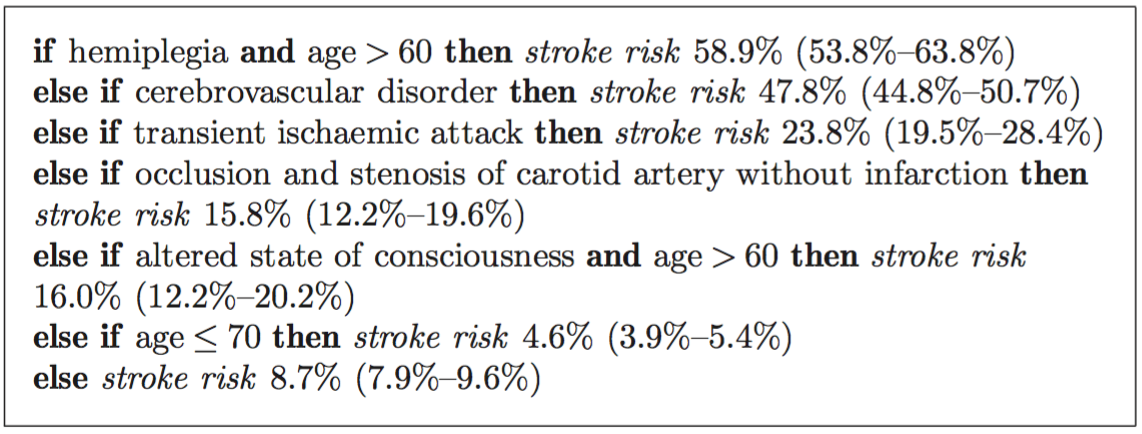
\includegraphics[width=0.9\textwidth]{figure/bayesian-rule-list}
  \caption{A decision list learned by the BRL algorithm \cite{letham2015stroke}.}
  \label{fig:bayesian-rule-list}
\end{figure}

\begin{figure}[tb]
  \centering
  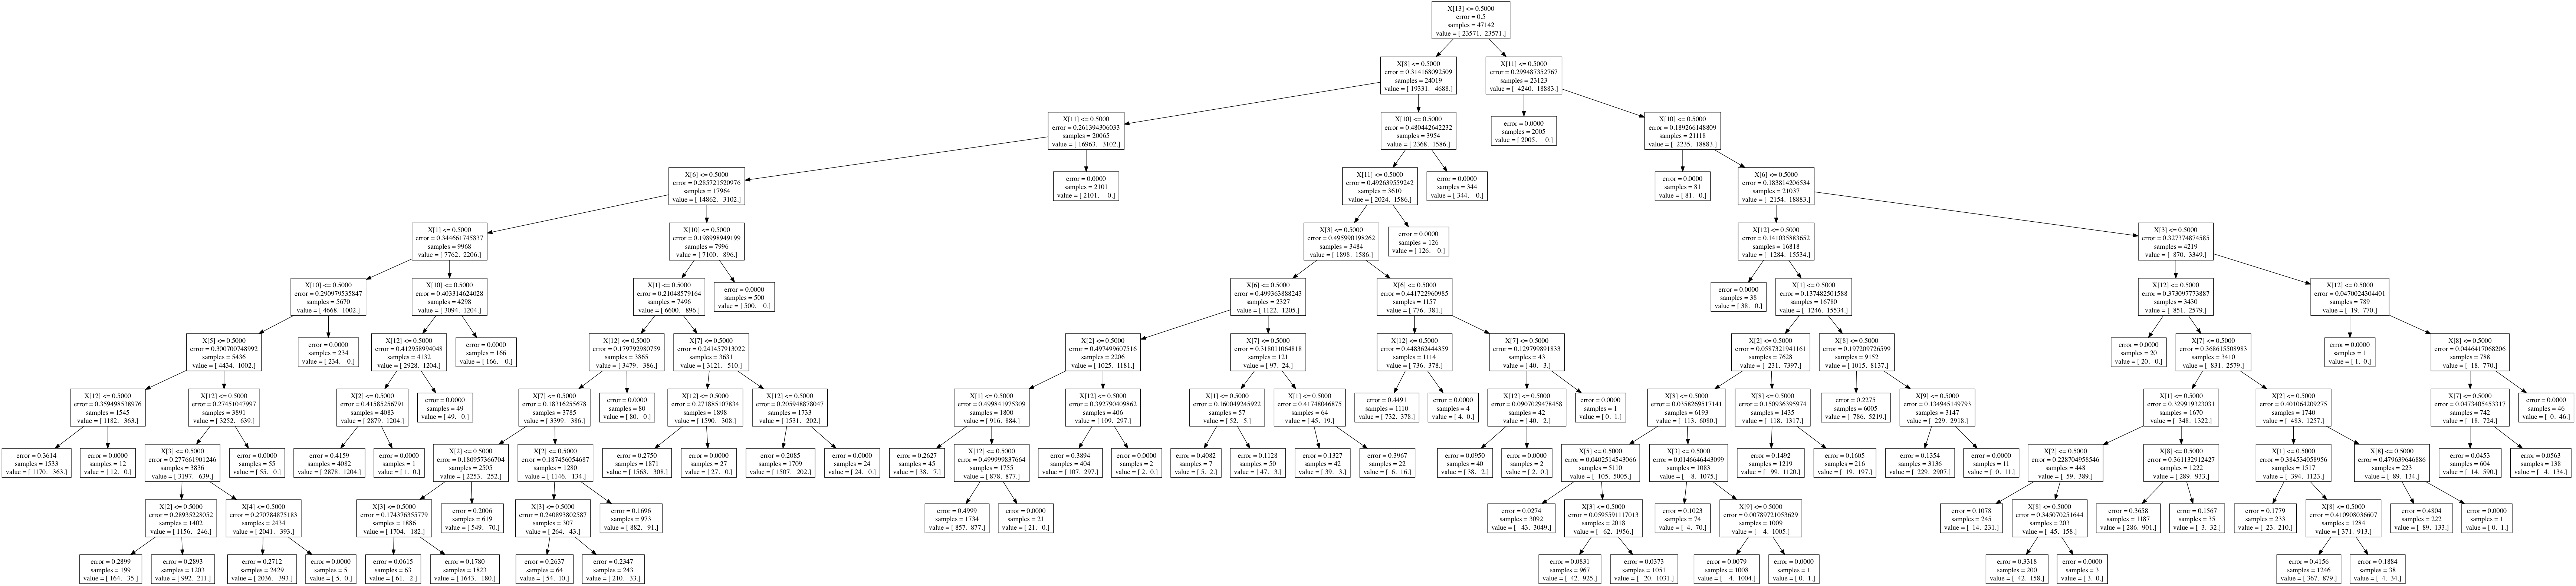
\includegraphics[width=1.0\textwidth]{figure/huge-tree}
  \caption[A decision tree with over one hundred nodes, which is hard to explain its reasoning.]{A decision tree with over one hundred nodes, which is hard to explain its reasoning\footnotemark.}
  \label{fig:huge-tree}
\end{figure}
\footnotetext{\url{https://umbrella.cisco.com/blog/2013/06/13/server-side-software-and-malware-analysis/}}

The most series problem of these interpretable models with easy-to-understand structures is the scalability. The performance of the rule-based models increases as the number of rules increases or the non-linearity increases. Although the rule-based models are easy to learn and understand at the first glance, it is intractable to understand the classifier as a whole when the number of nodes of rules grows up to a few hundred. An example is shown in \autoref{fig:huge-tree}.

\textbf{Others}. Except for rule-based models, there are a few other models with more complicated models are recognized to be interpretable.
One family of interpretable models worth noticing are the generalized linear models \cite{debock2010gam}, which are pervasive in statistics and finance. Although these models can have highly nonlinear computations, the additive relation between nonlinear functions of features is believed to be easy-to-understand. However, the generalized linear classifiers can also be hard to understand when their non-linearity increased to a certain extent. The other non-probabilistic family of classifiers is the $k$-nearest neighbors (kNN) classifiers, whose prediction can be easily understood by presenting the observation's $k$-nearest neighbors. Numerous work has been done to boost the performance the kNN classifiers, including weighted kNN with different kernels \cite{dudani1976weightedknn} and fuzzy kNN \cite{keller1985fuzzyknn}. The explainability of kNN classifiers may easily fail when there lack good neighbors for certain observations.

% \subsection{Learning Interpretable Representations}

% Instead of restricting the classifier to the combination of simple computations, some other work dedicates to learn more interpretable representations from the data. For example, Maier \etal [] learning causal knowledge from relational representations

% Features used by the model are easily interpretable.

% e.g. KNN


% Translation \cite{bahdanau2014translation}.
% Image Captioning \cite{xu15icml}.

\subsection{Learning Sparse Models}

As discussed above, the explainability often decreases as the complexity (\ie, number of parameters or nodes) of the model increases. Thus, we can improve the explainability by learning a sparser model with the same architecture. Two common strategies are used to learn a sparse model: simplifying a ``dense'' model through pruning or approximation; introducing sparsity as a prior to learn a sparse model from scratch. 
% These methods can also be regarded as model compressions, which reduce computation costs. 

% Note that learning sparse neural networks are not part of this category, since they focus on reducing the computation cost rather than explainability.

\textbf{Simplification}. The methods for simplifying classifiers are usually developed in a model-specific manner. Quinlan \cite{quinlan1987simplifying} summarizes four techniques for simplifying decision trees , \ie, cost-complexity pruning, reduced error pruning, pessimistic pruning and simplification to rule sets. Downs \etal \cite{downs2001simplifysvm} recognize and eliminate dependent support vectors while leaving the outputs of SVM unchanged. Liu \etal \cite{liu2015sparsecnn} use a sparse decomposition method to zero out redundant parameters in a CNN, achieving about 10-times speedup while only losing about 1\% accuracy. Though these methods can practically simplify classifiers and speed up computations, they do not directly provide explainability. A simplified SVM with fewer support vectors but utilizing a complicated kernel is still difficult to explain. A simplified decision tree with 200 nodes instead of 1,000 nodes is still hard to interpret.

\textbf{Learning from scratch}. To directly learn sparser models from scratch, Tipping \cite{tipping2001sparse} proposes a general Bayesian framework that treats sparsity as a prior and specialized this method on SVM. Instead of restricting the complexity of the parameters, Tan \etal \cite{tan2010sparsesvm} uses a 0-1 control variable to each input feature, and convert the learning to a mixed integer programming problem. The similar idea can be found in the sparse linear integer models proposed by Ustun \etal \cite{ustun2016supersparse}. Although these methods can learn sparse classifiers without losing much performance, they mainly focus on reducing the computation costs instead of providing explainability. They do not guarantee explainability if the classification problem is difficult.

In most cases, the efforts of developing more interpretable classifiers are tradeoffs between performance and explainability. For performance-critical applications, it is always difficult to train an interpretable classifier that does not need extra explanations.

% A common problem of these interpretable classifiers, either by using simple structures or by learning sparser models, is that their explainability depends on the data itself. If the inputs $\mathbf{x}$ are intrinsically difficult to explain,

\section{Explaining Complex Classifiers}

Generating explanations of a classifier without modifying the classifier itself is preferred when the underlying model is already too complicated, \eg, neural networks and SVMs, and we don't want to sacrifice performance. There is also no common-recognized definition for what an \textbf{explanation} of a classifier is. Most existing work uses a subset or a weighted subset of input features to explain a single prediction of a classifier, \eg, a mask over the input image, a heatmap with the same size as the input image, a bag of words or categorical fields. Some work \cite{ribeiro2016kdd} proposed to induct a simpler classifier (\eg, linear classifier) as the explanation of a prediction. Here we only discuss explanations for complex classifiers. Thus, illustrative diagrams for simple classifiers are not included here.

In cognitive science, explanations are characterized as arguments that demonstrating all or a subset of the causes of the \textbf{explanandum} (the subject being explained), usually following deductions from natural laws or empirical conditions \cite{hempel1948explanation,lombrozo2006explanation}. Here we give a general definition: 

\textbf{Explanations of a classifier} are the human-understandable representations that identify the causes of the classifier's prediction(s). A typical form of human-understandable representations is the visualization. As introduced in \autoref{sec:classifier-classification}, a classifier can be regarded as a function $f$, which is in general learned from a training dataset $\mathcal{D}$, specified by learned parameters $\theta$. Thus, the \textbf{causes} can be traced to 1) parts of the training data $\mathcal{D}$, 2) parts of the parameters $\theta$ as some components of the classifier, or 3) parts of the input, $x$, of a prediction or predictions. 

If an explanation is provided to explain $f$'s prediction in a small region around a given input point $\mathbf{x}$, we call it as a \textbf{local explanation}. If it is generated to explain $f$ on the whole input space $\mathcal{X}$ in general or as a summary, we call it as a \textbf{global explanation}. Sometimes, we also want to have an intermediate \textbf{subset explanation} that is performed on a subset $\mathcal{S}$ of $\mathcal{X}$, in which the inputs share some common features. 
%The global explanation can actually be regarded as a extreme case of subset explanation, where $\mathcal{S}=\mathcal{X}$. 
Next, we discuss the related work on explanations of classifiers based on the above taxonomy. 

%They are viewed as the central to our sense of understanding and the currency in which we exchange concepts \cite{lombrozo2006explanation}.

% \subsection{Definitions of Explanation}

% A review of how previous work define explanations in machine learning.

% General: ML:\cite{doshi-velez2017interpretableml}. Cognitive:\cite{lombrozo2006explanation}

% Data-type specific definitions: image-based, text-based, categorical data.

% Some other work focuses on explaining the model itself (the mechanism, compositions of the model) to facilitate the understanding and diagnosing of the model.

% To summarize, no agreed definition of explanation of classifier exists. Here we give a general definition...Next we give problem specific definitions.

% Learned from surveying the literature, we separate the problem of explaining classifiers into two sub-tasks: explaining the predictions of classifiers (instance-level); explaining the classifier itself (model-level).

% For each sub-tasks, the existing methods can be divided into two types: model-aware explanations and model-unaware explanations.


\subsection{Local Explanations}

As we have discussed, the causes used in an explanation of a classifier can be the training data, model parameters, and inputs. For local explanation, the input $\mathbf{x}$ is always specified and used in the explanation. Depending on whether an explanation is generated directly using model's parameters or structures, we categorize local explanation methods into model-aware and model-unaware methods.

\begin{figure}[tb]
  \centering
  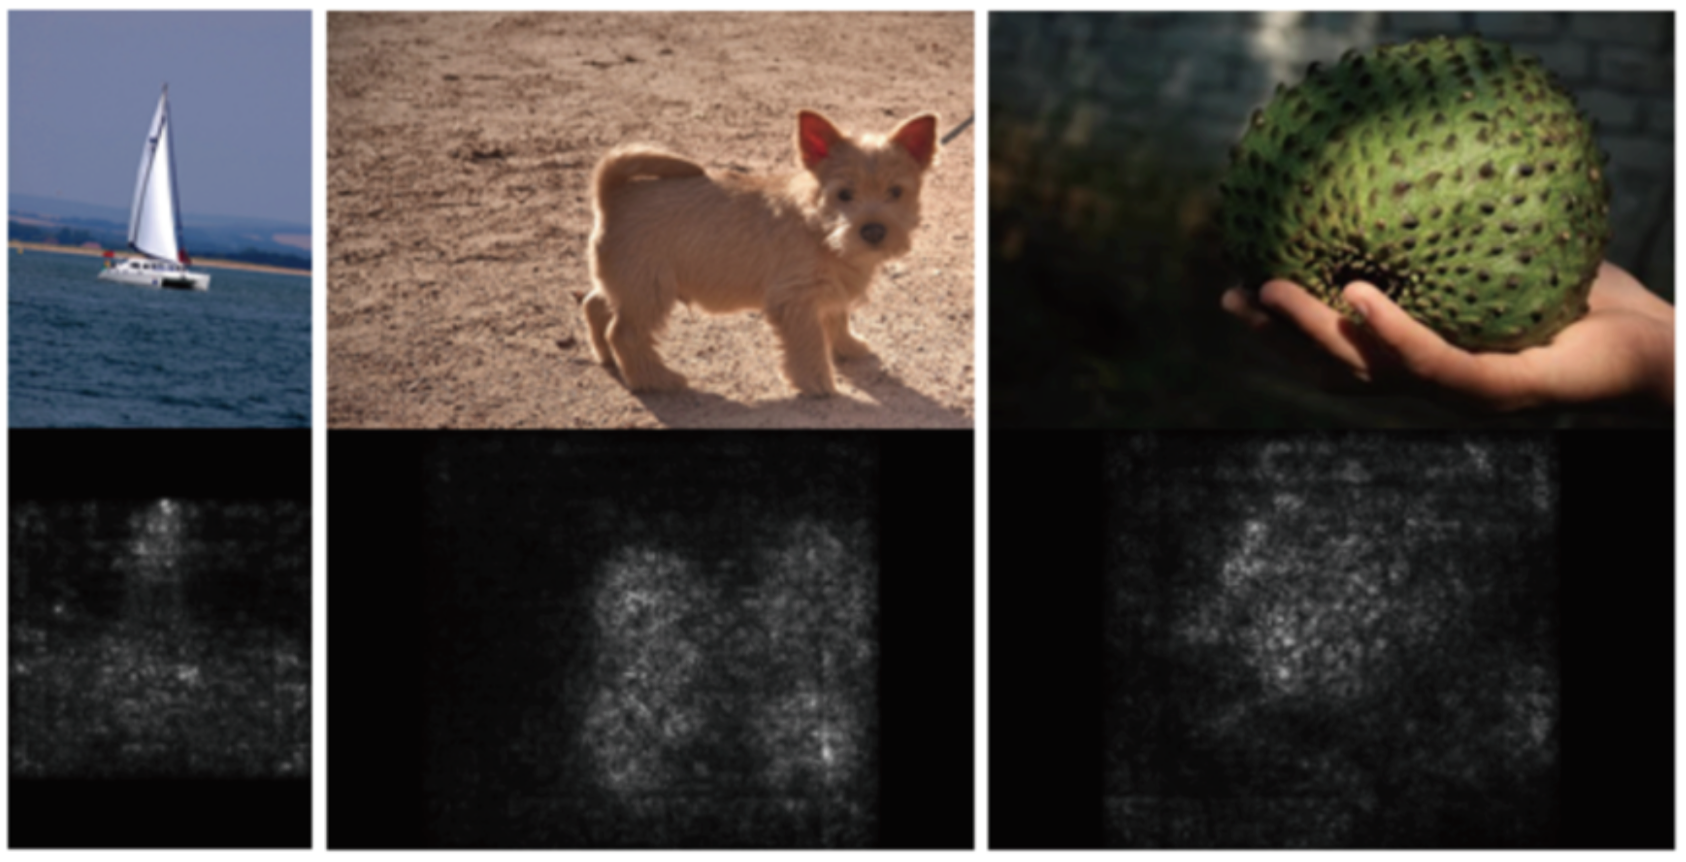
\includegraphics[width=1.0\textwidth]{figure/saliency-map}
  \caption{Images (first row) and their saliency maps (second row) for the top-1 predicted class in ILSVRC-2013 test images \cite{simonyan14saliency}.}
  \label{fig:saliency-map}
\end{figure}

\begin{figure}[tb]
  \centering
  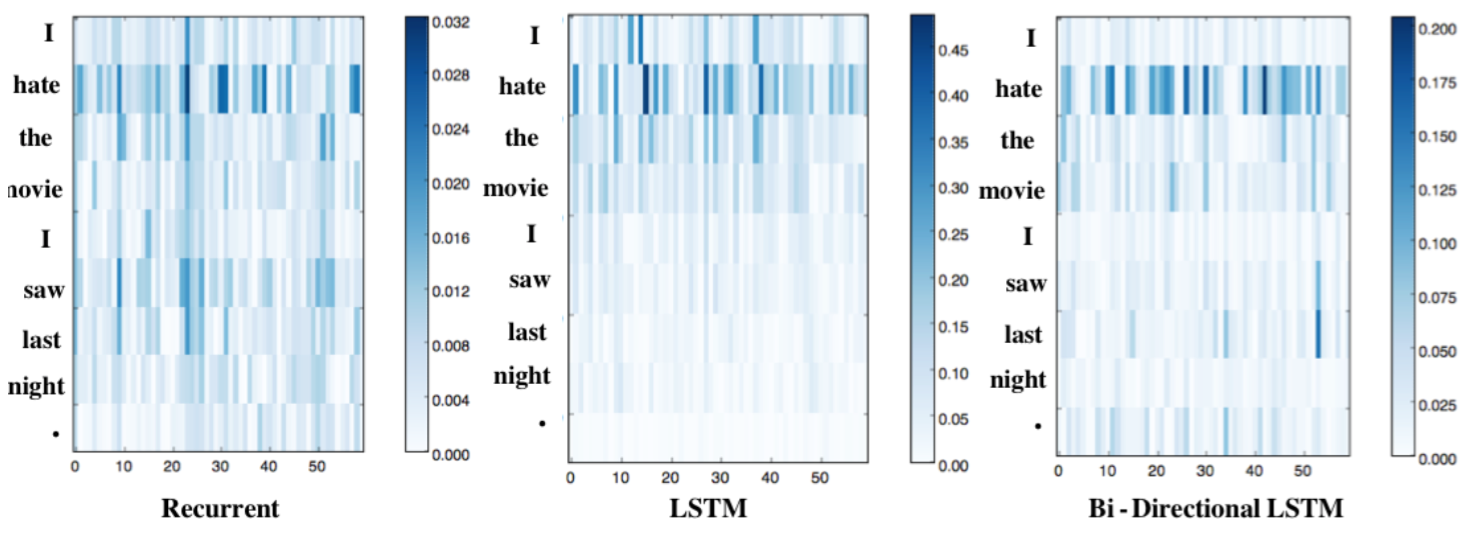
\includegraphics[width=1.0\textwidth]{figure/saliency-map-rnn}
  \caption{Saliency matrix maps for ``I hate the movie I saw last night.'' of three RNN sentiment classifiers. \textit{Left}: a vanilla RNN; \textit{Middle}: an LSTM; \textit{Right}: a bi-directional LSTM \cite{simonyan14saliency}.}
  \label{fig:saliency-map-rnn}
\end{figure}

\textbf{Model-unaware explanations} only require the input $\mathbf{x}$ and a computable $f$. Most work uses sensitivity or saliency-based techniques to derive explanations. Simonyan \etal \cite{simonyan14saliency} use the derivative of an image classifier $f_i$ w.r.t. the input image $\mathbf{x}$ as the saliency score of the class $i$, and map the score of each pixel to a saliency map as the explanation of $\mathbf{x}$. Li \etal \cite{li2016naccl-hlt} also calculate the derivative of a text sentiment RNN classifier w.r.t. the embeddings of an input sentence (which is a matrix), as shown in \autoref{fig:saliency-map-rnn}. The heatmap matrices are used as explanations for users to identify salient dimensions of the embedding vector and salient words that contribute the most to the prediction. Although these sensitivity-based methods are intuitive and can be efficiently approximated, their generated explanations are often noisy (as shown in \autoref{fig:saliency-map}), due to the high nonlinearity of the complicated classifier. Recently, Smilkov \etal \cite{smilkov2017smoothgrad} propose a random sampling technique to smooth the gradient, which achieves more meaningful visual explanations. However, this smoothing technique is computationally expensive and non-deterministic.

Instead of sensitivity analysis, some other work trains another model to explain the explanandum. Ribeiro \etal \cite{ribeiro2016kdd} approximate a complicated classifier locally using a simple linear classifier, and proceed to generate super-pixel patches as explanations. This method is actually similar to the gradient smoothing, since the training of the linear classifier is also done by sampling around the current input. Forming the problem as image captioning, Hendricks \etal \cite{hendricks16generate} use extra labeled explanation texts of images to train an explainer that generates explanatory texts of an image classifier. This method highly depends on the quality of text explanations labels, which require extra expensive labeling. Besides, it introduces another model, which is another potential explanandum that needs to explain.

% image data: \cite{simonyan14saliency,zeiler2014eccv,bach15plos,zintgraf17visualize}

% text data: \cite{karpathy16rnn,li2016naccl-hlt,martens2014explaindocument,arras2017rnn-sentiment}

\begin{figure}[tb]
  \centering
  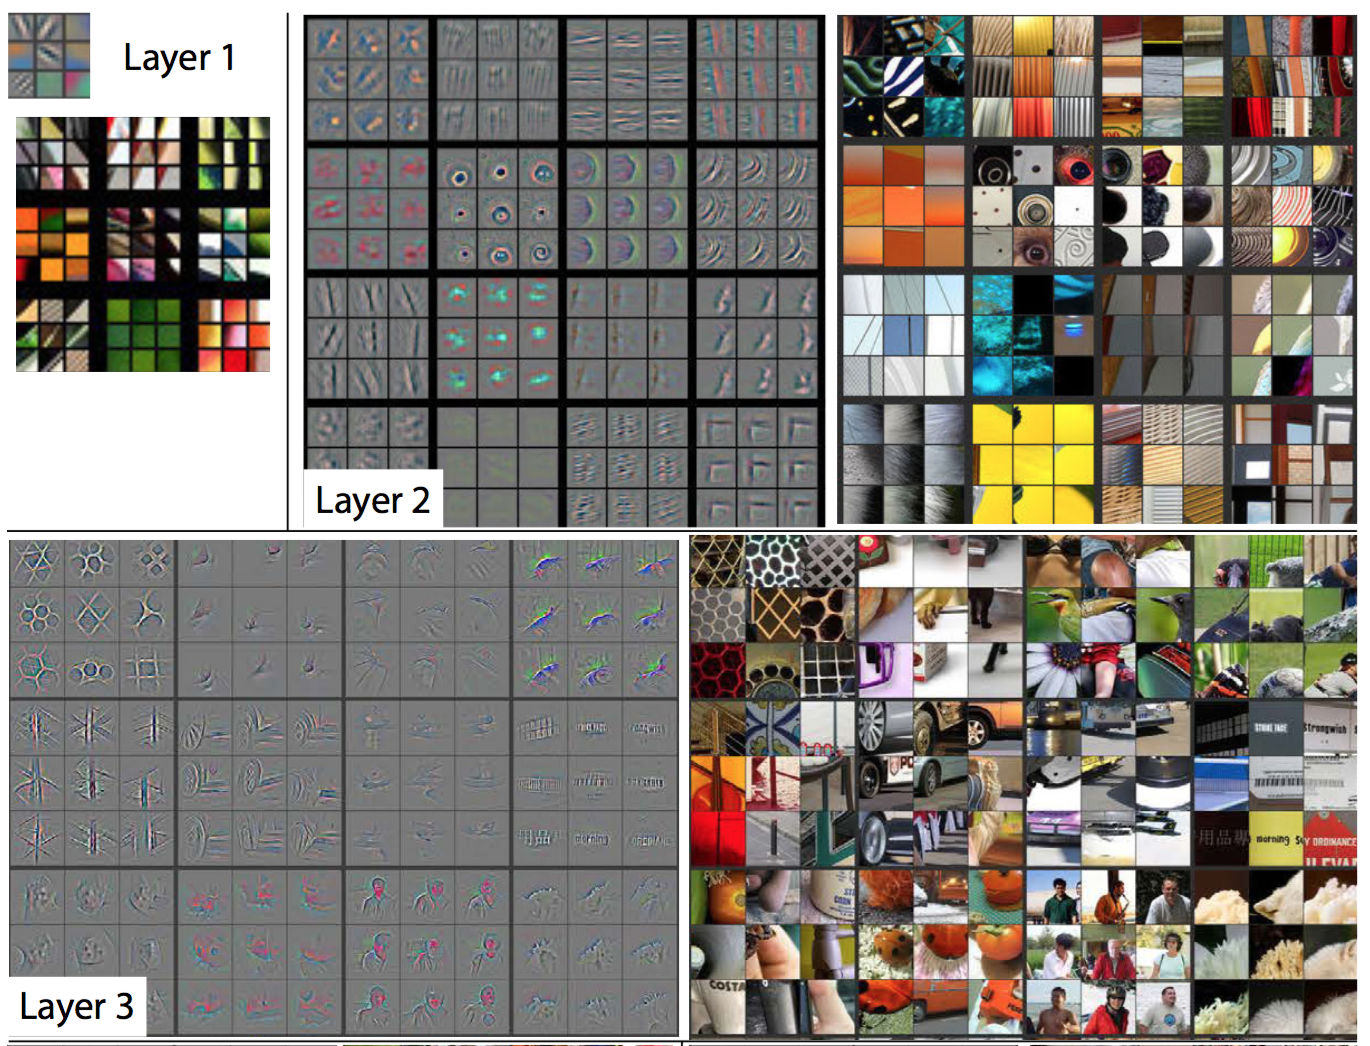
\includegraphics[width=1.0\textwidth]{figure/deconv}
  \caption{Visualization of a CNN generated using the de-convolution method \cite{zeiler2014eccv}. Gray images in the left are the top nine activations in a random subset of neurons across validation data, projected back to image space. In the right are corresponding image patches.}
  \label{fig:deconv}
\end{figure}

\textbf{Model-aware explanations} utilize another cause -- the parameters of the model, $\theta$, to amplify the information in the explanation. Zeiler and Fergus \cite{zeiler2014eccv} develop a de-convolution method that maps the outputs of a CNN classifier back to the input space, utilizing the inverse operations of different layers. The projected images \autoref{fig:deconv} can be used as an explanation of what different neurons are used for. Bach \etal \cite{bach15plos} use a layer-wise relevance propagation (LRP) that improves the sparsity of the image heatmap. Zintgraf \etal \cite{zintgraf17visualize} develop a visualization that highlights evidence for and against a prediction separately through prediction difference analysis. Murdoch and Szlam \cite{murdoch2017rule} decompose the output of an LSTM classifier into multiplicative contribution scores of input words and uses the scores to explain how important the words are for the prediction. Though these methods typically result in much better (sparse, meaningful) explanations than model-unaware methods, they are developed in a per-model manner, which are hard to generalize for other classifiers. There is a lack of general explanatory frameworks to guide and evaluate the development of model-aware methods. Flooded by the interest in deep learning, we can hardly find methods developed for classification models other than neural networks.

% Erhan \etal \cite{erhan2009techreport} developed the activation maximization method that generate 

Using the cause of training data for explanations has not attracted interest until recently. Koh and Liang propose a fast approximation of the influence function, which is a well-studied method in statistics. The influence functions can help identifying training points that are most responsible for a given prediction \cite{koh2017influencefunctions}, and thus can explain the prediction from the aspect of training data.
 
\subsection{Global Explanations}
The global explanations are not dependent on any specific inputs. A global explanation is actually a summary of the reasoning of how a classifier generally behaves. Unlike local explanations which are defined around a certain point, the global explanations are considered to be ill-posed and are much harder to achieve. Similarly to local explanations, we divide existing work into model-aware and model-unaware methods.

\textbf{Model-unaware explanations}. To our knowledge, very few methods have been proposed to generate global explanations for general classifiers. Ribeiro \etal \cite{ribeiro2016kdd} select a collection of representative local explanations and present to the users one local explanation at a time to give a global understanding. This method will easily fail when the dataset (training data) is too large. The users will not be able to remember a lot representative local explanations to form a global understanding.

% \cite{ribeiro2016kdd} Image and text, sampling instanc-level explanations

\textbf{Model-aware explanations}. The first attempt to understand a complex classifier globally is done by F{\'e}raud and Cl{\'e}rot \cite{feraud2002nn}. They partition the hidden representation space through clustering the representation of the whole training set, where each cluster represents a semantic concept learned by the classifier. To qualitatively understand a CNN, Erhan \etal \cite{erhan2009techreport} propose the activation maximization method. Each neuron in the CNN can be explained using an image patch that will maximize its activation. 
% Ming \etal \cite{ming2017vast} summarize the functions of different hidden units of an RNN classifier using collections of words through co-clustering and find interesting semantic clusters in the hidden state. 
To provide conceptual meanings of the explanation, Bau \etal \cite{bau2017netdissect} align hidden units with human-understandable concepts (objects) through a dissection process. However, these methods often require explorations over multiple nodes or neurons. The big picture is often neglected. Additionally, a common issue is that it is hard to compare these methods due to the lack of an evaluation framework.

% RNN: \cite{ming2017vast}

% CNN: \cite{bau2017netdissect} study interpretable units

% NN: \cite{feraud2002nn}

% \section{Research Issues}

In summary, there are two common strategies to make a classifier explainable. First, we develop simpler or sparser classifiers that can meet the performance requirements. Second, we build another human-understandable interface for explanation on top of a classifier. Both strategies are useful in different scenarios. 

However, an important, but neglected aspect of existing methods is the human. Few have paid attention to model human. Most of them study the classifiers and develop techniques for explainability and then argue that their methods help humans to understand the classifier, without studying how humans exactly response to the results generated by these techniques. 

Another related problem raised by Doshi-velez and Kim \cite{doshi-velez2017interpretableml} is the lack of the evaluation methods for explainability. Without a rigorous evaluation, it is hard to compare which method is better in a certain setting. It will also be infeasible to clarify the gap of current research and direction for future research.
% Address the problem of evaluation, and how other work evaluates.

\newpage